% TEMPLATE for Usenix papers, specifically to meet requirements of
%  USENIX '05
% originally a template for producing IEEE-format articles using LaTeX.
%   written by Matthew Ward, CS Department, Worcester Polytechnic Institute.
% adapted by David Beazley for his excellent SWIG paper in Proceedings,
%   Tcl 96
% turned into a smartass generic template by De Clarke, with thanks to
%   both the above pioneers
% use at your own risk.  Complaints to /dev/null.
% make it two column with no page numbering, default is 10 point

% Munged by Fred Douglis <douglis@research.att.com> 10/97 to separate
% the .sty file from the LaTeX source template, so that people can
% more easily include the .sty file into an existing document.  Also
% changed to more closely follow the style guidelines as represented
% by the Word sample file. 

% Note that since 2010, USENIX does not require endnotes. If you want
% foot of page notes, don't include the endnotes package in the 
% usepackage command, below.

% This version uses the latex2e styles, not the very ancient 2.09 stuff.
\documentclass[letterpaper,twocolumn,10pt]{article}
\usepackage{usenix,epsfig,endnotes,enumitem,multicol}
\begin{document}

%don't want date printed
\date{}

%make title bold and 14 pt font (Latex default is non-bold, 16 pt)
\title{\Large \bf RIPLE: Movie Recommendation and Imdb Score Prediction using Machine Learning}

%for single author (just remove % characters)
\author{
{\rm Michail G.\ Pachilakis}\\
csd3077@csd.uoc.gr
\and
{\rm Iordanis P. Xanthopoulos}\\
csd3161@csd.uoc.gr
% copy the following lines to add more authors
% \and
% {\rm Name}\\
%Name Institution
} % end author

\maketitle

% Use the following at camera-ready time to suppress page numbers.
% Comment it out when you first submit the paper for review.
\thispagestyle{empty}


\subsection*{Abstract}
\par As the number of movies released each year continuously grows, viewers are flooded with information about several new movie productions, making simple questions like "What movie should I see tonight?", really hard to answer. Also, production studios would like to know if a movie could be a commercial success before it comes out to theaters, in order to invest money in it.\par In this work, we provide  \textbf{i.} a simple question interface, so the users can find movies matching their criteria, \textbf{ii.} an interface to answer statistic related questions about any movies-related dataset and \textbf{iii.} predictions about a movie\textsc{\char13} s IMDB score, by using Machine Learning.\\
\\
\textbf{Keywords} Machine Learning; imdb; prediction; spark; statistics; recommendations


\section{Introduction}

\par Over the years, choosing which movie to watch has become an increasingly hard task. Every month, dozens of movies, from all over the world, are released and the average viewer, even though he may have a certain taste, is often overloaded by the amount of information presented to him via the websites or other sources of information. 
\par Nowadays, almost everyone heads over to imdb.com, in order to select which movie to see. It is most likely, the users will base their selection on its rating, which comes from the reviews of others, since going for one with a score of over 7.0 out of 10, is a safer choice and limits the possibility they will waste their time watching something that does not comply with their interests or simply is not good enough. Having filters that allows the user to find lists of possible recommendations, based on his preferred criteria, can be time-saving and remove the hustle of searching without having a certain goal in mind. In this paper, we present such filters, with which everyone can create the aforementioned lists, which are based on a decent-sized dataset, and save the user from the frustration of the endless browsing.
\par Moreover, the characteristics of a movie can contribute to its success or failure, which is represented by the rating users submit in movie websites and, in our case, imdb.com. With all that in mind, it is useful to predict the result of the movies rating, due to the fact it can ultimately determine, to a large extent, its overall popularity. Here, we show the implementation of a model that does just that, predicting a movie's rating, before its release.
\par Section 2, describes the datasets used for the creation of the filters and the ML model. Section 3, describes their implementation. Section 4, presents the results of the ML model, regarding its accuracy and compares it with implementations found in the literature. In Section 5, we come to a conclusion, as to our experiments and in Section 6, we give out our source code, since the whole project is open-source and part of a class for the university.

\section{Dataset}
\par The dataset was created at 2016 by Chuan Sun, who used it on an article at nycdatascience.com\cite{nyc} and can be found, copyright-free and free of charge, at Kaggle\cite{kaggle}. The dataset is consisted of 5043 lines, each line representing a movie, and 28 columns, depicting its characteristics. The size of the dataset is 579.78KB and the format of the data is text, containing both alpharithmetic and numeric values.\par Since the data are originated from IMDB, we do not expect any biases, regarding the scores and the validity of movie characteristics, such as the actors' lineup and the director. Still, even though the dataset has enough data for the small-scaled experiments we conducted, some of its flaws are mentioned by its creator and can create issues during the analysis setup, so we ought to point them out as well. In some cases, the columns have blank fields, which gave an error output, if left unhandled, during the construction of the ML model. The inflation factors are not taken into consideration, it goes without saying that 1000US dollars did not have the same value at 1920s as they do nowadays, and we do not take any particular actions regarding this matter, due to the high complexity of the conversion. \par Below, we present the 28 characteristics of the dataset, with a minor description for each one, as to its type and what it is about:

\begin{itemize}
\item \textbf{color}: Binary alpharithmetic variable, with possible values “Color” or “Black and White”.
\item \textbf{director\_name}: Categorical alpharithmetic variable, the director of the movie.
\item \textbf{num\_critic\_for\_reviews}: Numeric variable, how many reviews are written for the movie by critics.
\item \textbf{duration}: Numeric variable, how long the film lasts.
\item \textbf{director\_facebook\_likes}: Numeric variable, how many likes the director of the movie has on facebook.com.
\item \textbf{actor\_3\_facebook\_likes}: Numeric variable, how many likes the third actor (in lineup order) has on facebook.com .
\item \textbf{actor\_2\_name}: Categorical alpharithmetic variable, the name of the second actor (in lineup order).
\item \textbf{actor\_1\_facebook\_likes}: Numeric variable, the number of likes the first actor (protagonist) has on facebook.com .
\item \textbf{gross}: Continuous numeric variable, the total gross of the movie.
\item \textbf{genres}: Alpharithmetic variable, contains a number of predefined strings, such as Action, Adventure etc.
\item \textbf{actor\_1\_name}: Alpharithmetic variable, the fullname of the first actor (protagonist).
\item \textbf{movie\_title}: Alpharithmetic variable, the name of the movie.
\item \textbf{num\_voted\_users}: Numeric variable, the number of users who rated this film.
\item \textbf{cast\_total\_facebook\_likes}: Numeric variable, the number of likes of the whole cast in the facebook.com .
\item \textbf{actor\_3\_name}: Alpharithmetic variable, the full name of the third actor.
\item \textbf{plot\_keywords}: Alpharithmetic variable, the plot keywords, separated by lines "\textbar".
\item \textbf{movie\_imdb\_link}: Alpharithmetic variable, the IMDB link of the movie. 
\item \textbf{language}: Alpharithmetic variable, the main language that the actors speak in the movie.
\item \textbf{actor\_2\_facebook\_likes}: Numeric variable, the number of likes the second actor (in lineup order) has on facebook.com . 
\item \textbf{num\_user\_for\_reviews}: Numeric variable, the number of reviews written for the movie by users.
\item \textbf{face\_num\_in\_poster}: Numeric variable, the number of actor faces in the movie poster.
\item \textbf{movie\_facebook\_likes}: Numeric variable, the number of likes the movie has on facebook.com.
\item \textbf{country}: Categorical alpharithmetic variable, the name of the country where the movie was shot at.
\item \textbf{content\_rating}:  Categorical alpharithmetic variable, the content's age rating.
\item \textbf{budget}: Numeric variable, how much money the movie production cost.
\item \textbf{title\_year}: Numeric variable, the year the movie was released in cinemas.
\item \textbf{imdb\_score}: Numeric variable, the overall movie score in imdb.com.
\item \textbf{aspect\_ratio}: Numeric variable, the aspect ratio of the movie.
\end{itemize}

\begin{figure*}	
	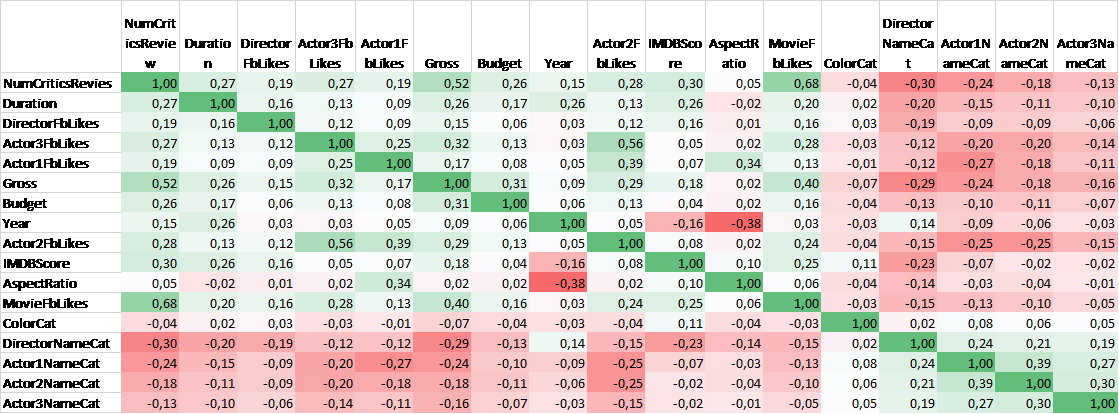
\includegraphics[width = \textwidth,height=6.2cm]{correlation_matrix_image}
	\caption{heatmap of the correlation matrix}
\end{figure*}

\section{Implementation}
We selected to implement three different functionalities. The first one targets mostly the movie production studios and is about movie score predictions. The other two are statistics about the movies, contained in the dataset and movie recommendations, which mostly target the viewers. 
\par For our implementation, we used Apache Spark\cite{spark} and the Scala programming language\cite{scala}. In the subsection 3.1 we describe the movie predictions implementation and in the subsection 3.2, the implementation of movies statistics and recommendations.

\subsection{Machine Learning}
Spark provided us with MLlib, a scalable machine learning library, which is consisted of common ML algorithms and utilities. Furthermore, it gave us access to spark.ml, which aims to provide a uniform set of high-level APIs that help users to create and tune practical ML pipelines. 

\par Firstly, we created a case class containing 28 fields, as many as the dataset features, and after parsing the initial dataset, we set every feature to its corresponding class field. We removed from the dataset movies containing commas in their titles, because, during splitting, they generated more features than they should, causing errors to the comma separated file.\par 

From our initial 28 features, we kept only those with a meaning to our predictions, so features like "Title", "IMDBLink", "Country" etc, were dropped. We removed 11 features, which, to our understanding, have the least effect on IMDB score prediction. \par 

Due to our dataset containing a mix of string, double and integer features, we had to transform our alpharithmetic ones to numeric. The package spark.ml has the StringIndexer function for that matter. StringIndexer converts String values into categorical indices which could be used by machine learning algorithms in spark.ml library.\par 

From our remaining features (17), we had to select only those that would positively affect the prediction of the movie's IMDB rating. To achieve this, we correlated our remaining features and excluded those that had a negative impact on the the "imdb\_score" feature. Again, the MLlib package provided us with the Statistics package, which contains the necessary functions for the feature correlation.\par 

In order to create our machine learning pipeline, we had to put together transformers to produce our output dataframe. We created a VectorSlicer, which takes a vector as input column and creates a new one, containing only the features that we chose from the original. We also created a StandardScaler, to scale a vector into one whose values are in similar scale, as well as a VectorAssembler, a feature transformer that merges multiple columns into a vector column.\par 

We initialized the Linear Regression Classifier estimator and then chained it with the VectorSlicer, StandardScaler and VectorAssembler transformers in the ML pipeline. When the pipeline is used to fit training data, the transformers and the estimator will apply on the dataframe, based on the sequence we defined.\par 

\subsection{Statistics and Recommendations}

For the Statistics and Recommendations, we used map and reduce functions. We took the same case class we described in the section 3.1 to create a RDD with 28 features named \textbf{parsedPointsRdd}. Afterwards, we applied filter and ordering functions on it, to produce the recommendations. For the statistics, we applied filter functions to the \textbf{parsedPointsRdd} and then calculated them. \par 

For the statistics we defined the following functions:
\noindent
{\bf \tt GreatMoviesStatistics\((\)):Double } \\ 

\noindent
{\bf \tt DirectorStatistics\((director:String\)):Double } \\ 

\noindent
{\bf \tt GenreStatistics\((genre:String\)):Double } \\ 

The \textbf{GreatMoviesStatistics} calculates the percentage of movies that have IMDB score above 8. These are the ones that are considered the best and everyone should probably watch them. The \textbf{DirectorStatistics} calculates the percentage of movies that a specific director has directed. The \textbf{GerneStatistics} estimates the percentage of movies included in a specific genre. \par


For the recommendations, we defined the following functions:

\noindent
{\bf \tt BestMoviesInCategory\((category:String\)) } \\

\noindent
{\bf \tt findTopTen  \((category:String,language:String,actor1name:String\)) } \\

\noindent
{\bf \tt findTitle\((category:String, language:String, actor1name:String, directorname:String\)) } \\

The \textbf{BestMoviesInCategory}, prints the top ten movies of a genre that is specified by the user. The \textbf{findTopTen} prints the top 10 movies based on the genre, their language and the protagonist's name, each of these arguments is user specified. Finally, the \textbf{findTitle} prints the titles of movies that match some user-specified criteria. The user can specify the genre, language, protagonist's and director's name. If some of those arguments cannot be filled by the user, they can be left blank, just by passing the empty string "" as argument. More than one movie can fit the selected criteria, so we limit the function so that it returns the first ten movie titles, in descending IMDB score order. \par

\section{Results}
In this section, we present our machine learning results and evaluate our methodology. We describe in depth the correlation process and discuss our evaluation.\par
After loading our dataset and creating our dataframe, containing the 28 movie features, we dropped the ones we thought they will have the least impact on the IMDB score feature. These features were: \texttt{"Genre"}, \texttt{"Title"}, \texttt{"NumVotedUsers"}, \texttt{"CastTotalFbLikes"}, \texttt{"FacesOnPoster"}, \texttt{"PlotKeywords"}, \texttt{"IMDBLink"}, \texttt{"NumUserReviews"}, \texttt{"Language"}, \texttt{"Country"} and \texttt{"ContentRating"}. From these features, some cannot have been created before the movie's release, such as \texttt{"NumVotedUsers"}, and others cannot affect its score, e.g. the \texttt{"IMDBLink"}.\par 

We also had to transform the dataframe, convert the String features into numeric ones. Then, we proceeded to the correlation, which was done using the \texttt{"Pearson"} method. In figure 1, we present the heatmap extracted by the features' correlation. The greener a cell is, the more positively it correlates with the feature in that row, and the redder a cell is, the more negative weight gives in the correlation. Looking at the \texttt{"IMDBScore"} row of the matrix, we found that features such as \texttt{"Year"}, \texttt{"Actor2Name"}, \texttt{"DirecotrName"}, \texttt{"Actor1Name"} and \texttt{"Actor3Name"} have a negative weight on the IMDB score so we dropped them.

Using \texttt{randomSplit} we split our dataframe to two datasets. A train dataset containing 80\% of the movies in our initial dataset and a test dataset containing the remaining 20\%. We produced our model by fitting the training data to our pipeline. The testing data will go though, afterwards, our model to produce the prediction results.\par 

To evaluate our data we created a val \texttt{RegressionEvaluator} which we fed with our previous predictions. The root mean square error (RMSE) we found, was 1.02 which, considering our features and that the rating scale is from 0 to 10, is acceptable.

We also tested another set of features to make predictions. Based on the Chuan Sun work on the movie predictions. This set included the following: "IMDBScore", "DirectorFbLikes", "Duration", "Actor1FbLikes", "Actor2FbLikes", "Actor3FbLikes", "FaceNumOnPostes", "Year", "Color", "Budget". Using our model, because we do not know exactly the parameters used in his, we had an RMSE of 1.04. 
\section{Conclusion}

In this work, we created a model to predict movie IMDb scores. We created an interface wherewith users can get statistics about movies from a dataset and can get recommendations about the ones they may be interested in. Our testing shows we can predict movie scores with good sharpness and in the future we aim to reduce even more our prediction error rate.  

\section{Availability}

You can download the code we used for the machine learning predictions, recommendations and statistics from

\begin{center}
{\tt https://github.com/mipach/imdb/tree/master/src}\\
\end{center}

You can run our code with little or no modifications at all, using Apache Spark. This code is under no license, so you can use it freely but remember to refer our work.

\begin{thebibliography}{9}
	\bibitem{nyc} 
	Chuan Sun.
	\\\texttt{http://blog.nycdatascience.com/student-works/
		machine-learning/movie-rating-prediction}
	
	\bibitem{kaggle} 
	Chuan Sun - Kaggle competition.
	\\\texttt{https://www.kaggle.com/deepmatrix/
		imdb-5000-movie-dataset}
	
	\bibitem{spark} 
	Apache Spark.
	\\\texttt{https://spark.apache.org}
	
	\bibitem{scala} 
	Scala Programming Language.
	\\\texttt{https://www.scala-lang.org}
\end{thebibliography}




\end{document}